%
% Anlagendesign
%
% @version 1.0
% @author dmayer
% @created 29. Dezember 2015

\setchapterpreamble[o]{%
\dictum[--- \textsc{Charles Eames}]{\Gun Design is the appropriate combination of materials in order to solve a problem. \Gob}}
\renewcommand{\chapterheadstartvskip}{\vspace*{2cm}}

\chapter{Anlagendesign}
\label{chap:anlagendesign}

\renewcommand{\chapterheadstartvskip}{\vspace*{-0.5cm}}

Ziel dieses Kapitel ist es, eine Anlage zur Raumtemperaturregelung für den Betrieb mit Modellprädiktiver Regelung zu konzipieren, zu konkretisieren und im letzten Schritt umzusetzen. Dazu werden zunächst die allgemeingültigen Anforderungen an eine Anlage analysiert und schließlich verschiedene Vorgaben von Seiten der Hochschule Karlsruhe spezifiziert und ergänzt. Im darauffolgenden Schritt wird eine Idee abgeleitet, die anschließend zu einem Konzept weiterentwickelt und in ein konkretes Anlagendesign umgesetzt wird. Einzelnen Anlagenteile und deren Funktionsweisen werden zunächst näher beschrieben und im Anschluss auf die realen Einsatzbedingungen ausgelegt. Abschließend wird die Installation und dabei aufgetretene Besonderheiten der Anlage erläutert.

\section{Analyse der Anforderungen}
\label{sec:anforderungen}

\subsection{Einsatzziele und Rahmenbedingungen}
Um die Anforderungen an eine Anlage zu bestimmen, die sich für die Anwendung mit Modellprädiktiver Regelung eignet, werden zunächst die Einsatzziele der Anlage definiert. Wie in Kapitel \ref{sec:motivation} erwähnt, ist die hier betrachtete Anlage als Teil einer großen Anlage gedacht, daher sollten die Einsatzziele kompatibel zueinander gewählt werden. Um die Kompatibilität zu gewährleisten, wurde mit den Projektverantwortlichen\footnote{In Person von Herrn \textsc{Adrian Bürger} und \textsc{Markus Bohlayer}} der Forschung im Bereich solarer Anwendungen an der Hochschule Karlsruhe gemeinsam konkrete Einsatzziele der Anlage erarbeitet. Als Ergebnis wurden die folgenden konkreten Ziele vereinbart:
 
\begin{itemize}
	\item Die Einarbeitung in die Thematiken Modellbildung, Kommunikation von technischen Systemen und Modellprädiktive Regelung soll durch eine praktisches Anwendung unterstützt werden.
	\item Es soll Know-how im Bereich der Kommunikation von technischen Systemen aufgebaut werden, insbesondere im Umgang mit der Software, der Hardware und den zahlreichen Schnittstellen.
	\item Die Anlage soll eine hohe Funktionalität und Robustheit gegenüber Fehlern und Beschädigungen vorweisen, da bei der Einarbeitung eine erhöhte Wahrscheinlichkeit der Fehlbedienung besteht und Schäden dadurch vermieden werden sollen.
	\item Es soll ein Vergleich verschiedener Methodiken beim Einsatz von Modellprädiktiver Regelung ermöglicht werden.
	\item Außerdem soll ein Vergleich von Ergebnissen bei der Variation von Steuerungsparametern sowie beim Einsatz verschiedener Steuerungs- und Regelungsalgorithmen ermöglicht werden.
	\item Die Anlage soll flexibel ansteuerbar und erweiterbar sein, sodass der Grad der Komplexität verändert werden kann.
	\item Die Anlage soll ermöglichen den Einfluss der Sonneneinstrahlung auf die Raumtemperatur zu untersuchen.
	\item Im Rahmen der Anwendungsforschung soll das Modell des betrachteten Raumes zur Temperaturregelung möglichst nahe der Realität entsprechen.
\end{itemize}

Zusammenfassend lässt sich festhalten, dass die Anlage als Forschungsumgebung für Entwicklungs-, Test- und Anwendungszwecke von verschiedenen Steuerungen und Regelungen dienen soll.

Neben den oben genannten Einsatzzielen wurden von Seiten der Hochschule Karlsruhe\footnote{In Person von Frau Professor \textsc{Angelika Altmann-Dieses}, Herrn Professor \textsc{Marco Braun} und Herrn \textsc{Adrian Bürger}} weitere Rahmenbedingungen definiert, die im Folgenden dargestellt sind:

\begin{itemize}
	\item Der Raum K004b im K Gebäude der Hochschule Karlsruhe wird zur Installation der Anlage und Einrichtung der Forschungsumgebung zur Verfügung gestellt.
	\item Die Installation der Anlage muss mit minimalem baulichem und finanziellem Aufwand realisierbar sein.
	\item Für die Kommunikation zwischen den Anlageteilen soll die Modbus Kommunikationstechnologie mit mindestens zwei verschiedenen Übertragungsprotokollen genutzt werden.
	\item Die Modellprädiktive Regelung soll mit Hilfe der Plattform JModelica.org erfolgen.
\end{itemize}

\subsection{Definition der Anforderungen}

Aus den Einsatzziele und Rahmenbedingungen lassen sich die Anforderungen an die Anlage ableiten, welche im Nachfolgenden explizit aufgeführt sind. Aus Gründen der Übersichtlichkeit sind die wichtigsten in der nachfolgenden Tabelle \ref{tab:anforderungen_umgebung} zusammengefasst.


\begin{table}[H]
\centering
\small
\renewcommand{\arraystretch}{1.3}
\begin{tabularx}{1\textwidth}{m{0.35\textwidth}m{0.58\textwidth}}

\toprule

\textbf{Einsatzziele und} & \multirow{2}{\hsize}{\textbf{Anforderungen}} \\ 
\textbf{Rahmenbedingungen} & \\

\cmidrule[0.5pt](r{0.25em}){1-1} 
\cmidrule[0.5pt](l{0.25em}){2-2}

\addlinespace[1mm]
Raum K004b als Umgebung  & \multirow{3}{\hsize}{
\begin{minipage}[t]{0.57\textwidth}
\begin{itemize}[itemsep=0pt,topsep=0pt,leftmargin=5mm]
	\item Anpassen der Anlage an Raum K004b.
	\item Nutzen bestehender Heizkörper anstatt einer Klimatisierung des Raumes. 
	\item Die Anlage soll auf die wesentlichen Funktionalitäten und eine minimale Anzahl an Komponenten beschränkt sein. 
\end{itemize}
\end{minipage}
}
 \\
	
\cmidrule[0.1pt](lr{2em}){1-1} 
\addlinespace[1mm] Minimaler baulicher Aufwand & \\

\cmidrule[0.1pt](lr{2em}){1-1} 
\addlinespace[1mm] Minimaler finanzieller \newline Aufwand &\\ 



\cmidrule[0.5pt](r{0.25em}){1-1} 
\cmidrule[0.5pt](l{0.25em}){2-2}

\addlinespace[1mm] Modellprädiktive Regelung mit JModelica.org und CasADi \newline & \multirow{3}{\hsize}{
\begin{minipage}[t]{0.57\textwidth}
\begin{itemize}[itemsep=0pt,topsep=0pt,leftmargin=5mm]
\item Die Modellbildung erfolgt in Modelica.
\item Die Ansteuerung und Kommunikation innerhalb der Anlage soll in Python stattfinden.
\item Die Kommunikation der Anlage erfolgt gemäß den Modbus~RTU und TCP Protokollspezifikationen.
\item Die Ansteuerung der Anlage soll innerhalb des gesamten lokalen Netzwerks über Modbus~TCP möglich sein.
\end{itemize}
\end{minipage}
}  \\

\cmidrule[0.1pt](lr{2em}){1-1}
\addlinespace[1mm] Einsatz der Modbus \newline Kommunikationstechnologie \newline 	& 		\\

\cmidrule[0.1pt](lr{2em}){1-1}
\addlinespace[1mm] Flexible Ansteuerung der Anlage \newline & \\

\cmidrule[0.5pt](r{0.25em}){1-1} 
\cmidrule[0.5pt](l{0.25em}){2-2}

Einarbeitung in die Thematiken:
\begin{minipage}[t]{0.34\textwidth}
\begin{itemize}[itemsep=0pt,topsep=0pt,leftmargin=4mm]
	\item Modellbildung
	\item Kommunikation technischer \newline Systeme
	\item Modellprädiktive Regelung
\end{itemize}
\end{minipage}
 	& \multirow{2}{\hsize}{
\begin{minipage}[t]{0.57\textwidth}
\begin{itemize}[itemsep=0pt,topsep=0pt,leftmargin=5mm]
	\item Komplexität ist notwendig, sie darf jedoch nicht zu hoch sein.
	\item Eine klare Struktur mitsamt einer scharfen Trennung ist erwünscht. Diese soll durch wenige thematische Überschneidungen erreicht werden.
\end{itemize}
\end{minipage}
}  \\

\cmidrule[0.1pt](lr{2em}){1-1} 

Know-how für Kommunikation \newline technischer Systeme 	&		\\

\cmidrule[0.5pt](r{0.25em}){1-1} 
\cmidrule[0.5pt](l{0.25em}){2-2}

Vergleich von Ergebnissen durch:
\begin{minipage}[t]{0.34\textwidth}
\begin{itemize}[itemsep=0pt,topsep=1pt,leftmargin=4mm]
	\item Die Variation von \newline Steuerungsparametern
	\item Den Verwendung verschiedener \newline Regelungsmethodiken
	\item Den Einsatz verschiedener\newline Algorithmen.
\end{itemize}
\end{minipage}

& \multirow{3}{\hsize}{
\begin{minipage}[t]{0.57\textwidth}
\begin{itemize}[itemsep=0pt,topsep=0pt,leftmargin=5mm]
\item Die Reaktion des Systems soll einfach und zugleich kostengünstig erfasst werden können.
\item Einfachen robusten Bauteile sollen zum Einsatz kommen.
\item Ziel ist die Erstellung eines wartungsarmen Systems.
\item Das Systems soll modular und ohne großen Aufwand für weitere Schritte erweiterbar sein.
\end{itemize}
\end{minipage}
}  \\

\cmidrule[0.1pt](lr{2em}){1-1} 

Hohe Funktionalität und \newline Robustheit & \\

\cmidrule[0.1pt](lr{2em}){1-1} 

Erweiterbarkeit der Anlage
 &  \\

\bottomrule
\end{tabularx}
\caption{Umsetzung der Ziele in Anforderungen der Anlage}
\label{tab:anforderungen_umgebung}
\end{table}

Die grundlegendste Anforderung der Planung, ist die Anpassung an die Gegebenheiten des Raumes K004b, welche in \ref{fig:skizzek004a} skizziert sind. Der Raum befindet sich auf dem Campus der Hochschule Karlsruhe, an der südwestlichen Ecke des K~Gebäudes im Erdgeschoss. Die südliche und westliche Wand teilt sich der Raum mit der Außenumgebung und wird daher im Folgenden als Außenwand bezeichnet. Die östliche und nördliche Wand sowie die Decke und der Boden des Raumes grenzen an weitere Innenräume des K~Gebäudes. In der südlichen Außenwand ist eine Fensterfront mit Jalousien eingebaut, direkt darunter ist ein Heizkörper installiert.

\begin{figure}
\centering
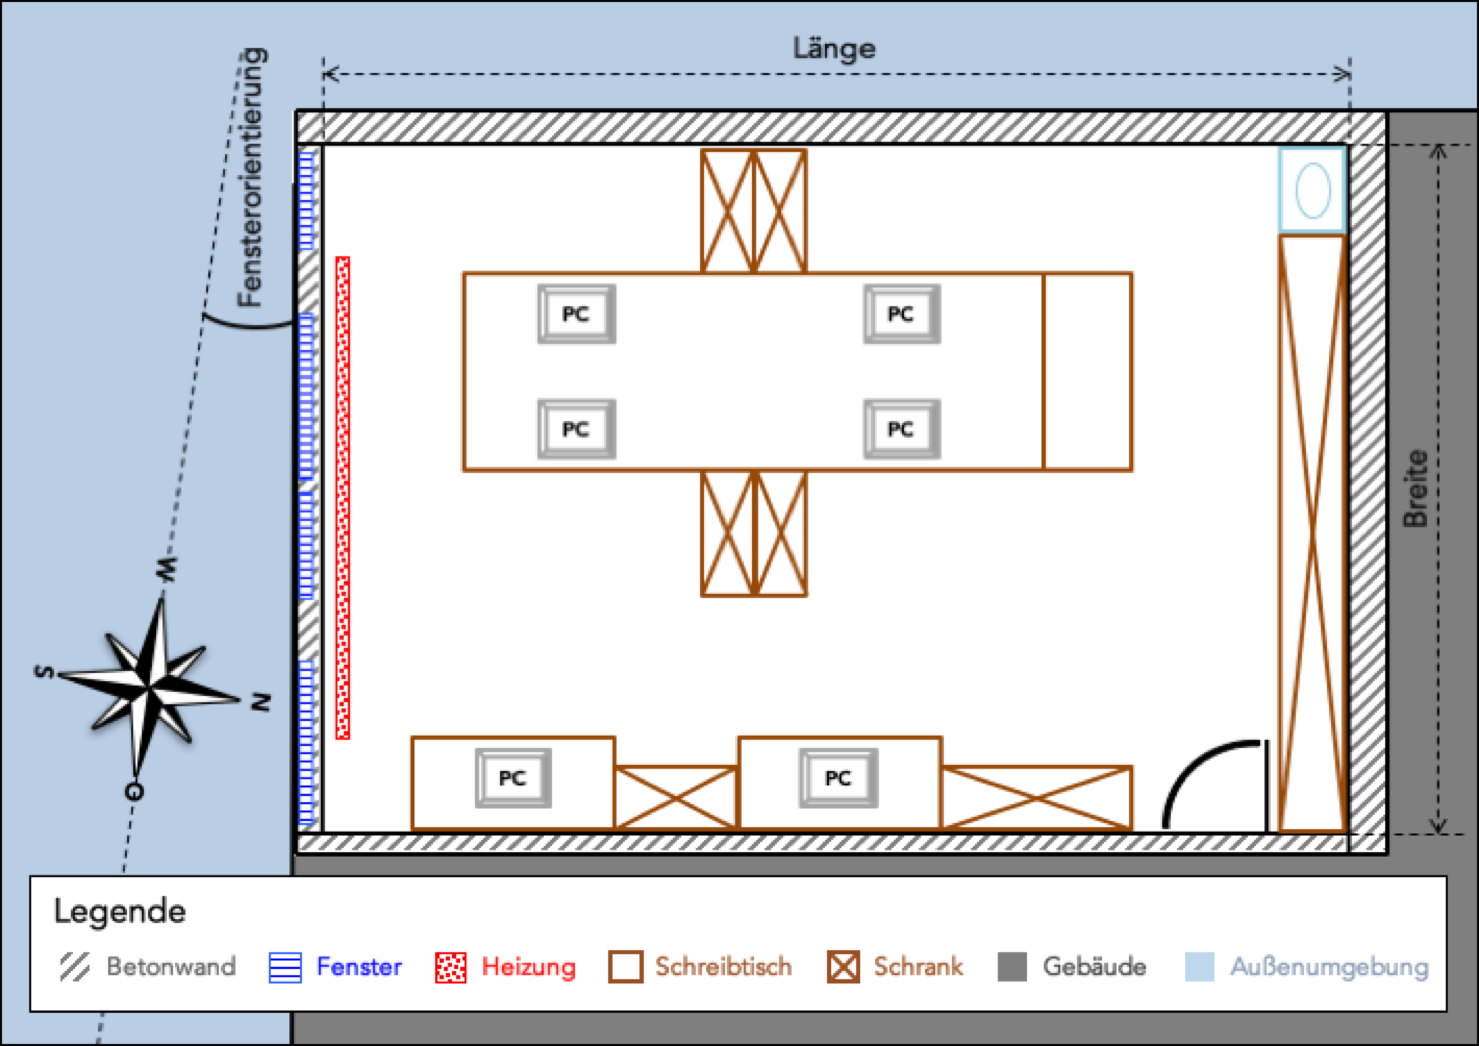
\includegraphics[width=\textwidth]{abbildungen/20160102_k004a}
\caption[Raumskizze K004b vom K Gebäude der Hochschule Karlsruhe -- Technik und Wirtschaft]{Raumskizze K004b vom K Gebäude der Hochschule Karlsruhe -- Technik und Wirtschaft}
\label{fig:skizzek004a}
\end{figure}

Durch die Raumwahl werden bereits zwei wichtige Anforderungen erfüllt, denn durch die Fensterfront kann der Einfluss der Sonneneinstrahlung auf die Raumtemperatur untersucht werden. Darüber hinaus kann der bestehende Heizkörper in die Anlage integriert werden und so einen minimalen baulichen Aufwand sicherstellen. Da eine Klimatisierung zur Raumtemperaturregelung mit einem erheblichen finanziellen und baulichen Aufwand verbunden wäre, kann diese zunächst ausgeschlossen werden. Um der Forderung nach einer erweiterbaren Anlage nachzukommen, soll bei der Planung ein möglicher Nachrüstungsvorgang durch eine Klimatisierung und eine Ansteuerung der Jalousien trotz alledem berücksichtigt werden.

Der Raum K004b wird als Büro von wissenschaftlichen Mitarbeitern der Hochschule Kalrsruhe genutzt, daher befinden sich darin, wie in \ref{fig:skizzek004a} abgebildet, sechs Computerarbeitsplätze und das übliche Büro-Mobiliar. Durch  den Einfluss von Mensch und Rechner, sogenannten Störgrößen welche im Modell berücksichtigt werden müssen, wird die Anforderung einer möglichst anwendungsnahen Umgebung erfüllt.

Als weitere restriktive Vorgabe soll die Modellprädiktive Regelung unter Zuhilfenahme der Plattform \textsc{JModelica.org} erfolgen. \textsc{JModelica.org} ist eine kostenlose Open-Source Plattform	 zur Analyse, Simulation und Optimierung von komplexen, dynamischen Systemen, die auf der Modellierungssprache Modelica basiert. Aufbauend auf den mathematischen Modellen physikalischer Systeme in Modelica, lassen sich, dank der Unterstützung der Spracherweiterung Optimica, Optimierungsprobleme durch einfache Konstrukte das Optimierungsintervall, die Kostenfunktion und die Nebenbedingungen einfach formulieren. JModelica.org wird über eine Python Nutzerschnittstelle genutzt und besitzt eine eigene Klasse für die Modellprädiktive Regelung, welche bisher noch experimenteller Art ist \cite[S.~1f.]{jmod15}.
Der Compiler kann die Modelle und Optimierungsprobleme in verschiedene Formate übersetzen. Zum einen in einen direkt ausführbaren C Code, der die Modellgleichungen und Optimierungsparameter enthält, und ein XML Code, der die Meta-Daten des Modells enthält. Zum anderen kann das Modell in ein \textit{OptimizationProblem} Objekt transferiert werden, welches eine symbolische Repräsentation des Optimierungsproblems darstellt \cite[S.~12ff.]{jmod15}.

Die \textit{OptimizationProblem} Objekte können anschließend direkt mit den Optimierungswerkzeugen von \textsc{CasADi} bearbeitet und damit zur Lösung des Optimierungsproblems eingesetzt werden. \textsc{CasADi} ist ein Open-Source Softwaretool, das einzelne Bausteine für die numerische Optimierung im Allgemeinen und für die Optimalsteuerung im Speziellen zur Verfügung stellt. Es eignet sich besonders gut für die gradientenbasierte numerische Optimierung von nichtlinearen Problemen aufgrund seiner effizienten Ableitungserzeugung durch die Algorithmische Differentiation und der Möglichkeit zur Integration von gewöhnlichen Differenzialgleichungen. Die Interaktion mit dem Nutzer soll aus Gründen der Stabilität über die Schnittstelle in Python erfolgen \cite[S.~5f.]{casadi}.
Daraus lassen sich weitere Anforderungen an das Modell ableiten, die in Kapitel \ref{chap:modellbildung} näher erläutert werden.

%Until here fine

Die vorgegebene Softwareplattform zur Modellprädiktiven Regelung und deren einzelne Komponenten besitzen allesamt eine Schnittstelle für Python, daher liegt es nahe, dass sowohl die Ansteuerung als auch die Kommunikation der gesamten Anlage in Python erfolgen. Python eignet sich hervorragend für diese Aufgaben, da es frei erhältlich ist und einen modularen Aufbau vorweist. Durch die Open-Source Lizenzierung ist die Programmiersprache frei nutzbar und bietet sowohl durch ihre Standardbibliothek als auch durch eine Vielzahl an von Nutzern entwickelten Bibliotheken, sogenannten Paketen, unzählige Anwendungsmöglichkeiten. Ein Beispiel für ein derartiges Paket ist das pysolar Paket, das im Rahmen der Modellbildung eine Umrechnung der an einem Fenster gemessenen in die wirkende Solarstrahlung ermöglicht \cite[S.~2f.]{python}.

Der Vorgabe der Modbus Kommunikationsprotokolle für die Kommunikation ist von ebenfalls von großer Relevanz, da die komplementäre Forschungsanlage zur solaren Klimatisierung dasselbe Kommunikationsprotokoll unterstützt und durch die gewonnenen Erkenntnisse eine beschleunigte Inbetriebnahme erfolgen kann. Um das Know-how breit zu fächern, sollen die beiden Modbus RTU und Modbus TCP Protokolle Anwendung finden. Außerdem soll das Kommunikationsnetzwerk aus mehreren Subnetzwerken aufgebaut sein, die durch verschiedene elektrische und mechanische Schnittstellen implementiert werden. Für die Kommunikation über Modbus werden in den Python Paketen pymodbus, minimalmodbus und modbus-tk bereits Bausteine zur Verfügung gestellt.

Die Anlage sollte einen möglichst geringen Komplexitätsgrad aufweisen, damit eine Einarbeitung in die einzelnen Themengebiete der Modellbildung, der Kommunikation von technischen Systemen und der Modellprädiktive Regelung mit einem überschaubaren Aufwand ermöglicht wird. Dies soll durch eine klare Abgrenzung der verschiedenen Anlagenteile und deren Funktionen, wie auch durch die Aufbaustruktur der Anlage erreicht werden. Im Gegensatz hierzu steht die Forderung nach dem Aufbau von Know-how auf dem Gebiet der Kommunikation technischer Systeme. Es muss daher ein Kompromiss zwischen Verständlichkeit und Komplexität gefunden werden. Um beiden Forderungen gerecht zu werden, findet die Kommunikation der Anlageteile ausschließlich über Modbus und unter Nutzung von verschiedenen Hard- und Software-Schnittstellen statt. Dadurch ist es möglich bereits erste Erfahrungen zu sammeln, die für die Inbetriebnahme der solaren Klimatisierungsanlage hilfreich sind.
Um eine Vergleichbarkeit von Ergebnissen zu gewährleisten, soll das System auf eine Veränderung der Steuergrößen eine schnelle\footnote{Im Kontrast zu den langsamen Reaktionen der solaren Klimatisierungsanlage, welche im oberen Minutenbereich liegen, bedeutet schnell in diesem Kontext im unteren Minutenbereich.} und zugleich unmittelbar messbare Reaktion zeigen. 
Daraus lässt sich folgern, dass die Aktorik ohne zeitliche Verzögerung auf Steuersignale ansprechen und die gesamte Anlage einen unmittelbaren Einfluss auf die vorherrschende Raumtemperatur haben soll. 
Die Messung der Raumtemperatur kann mithilfe von handelsüblichen Temperatursensoren erfolgen. Diese erfüllen die vorgegebenen Anforderungen der Hochschule Karlsruhe, da sie keinen allzu großen technischen und monetären Aufwand darstellen.

Als Basis für fortführende wissenschaftliche Tätigkeiten soll ein möglichst fehlerfreies System mit hoher Funktionalität erschaffen werden, sodass Fehlerquellen innerhalb des Systems von Vornherein ausgeschlossen werden können und damit nicht den Fokus von den eigentliche Forschungsaktivitäten lenken.
Zusätzlich ist eine hohe Robustheit der Anlage gegenüber Bedienungsfehlern und Beschädigungen erforderlich, da sie für Test- und Entwicklungszwecke genutzt werden soll. Dies lässt sich durch den Einsatz von wartungsarmen, einfachen und robusten Bauteile sowie den Aufbau der Anlage berücksichtigen und steht zugleich im Einklang mit der Forderung nach einer minimalen finanziellen Belastung.

Python stellt, wie bereits erwähnt, Schnittstellen und Funktionalitäten für die Aufgaben der Anlage zur Verfügung. Darüberhinaus bietet sich Python, durch ihre weitgehende Unabhängigkeit vom Betriebssystem, als zentrales Steuerungstool an. Hierdurch ist es einem nachfolgenden Schritt möglich einen Controller durch einen vergleichsweise günstigen Einplatinenrechner, wie beispielsweise durch einen Raspberry Pi, zu realisieren. Aus den eben genannten Gründen basiert die folgende Planung und Auslegung der Anlage auf einer zentralen Steuerung in Python.

\section{Idee und Ziel der Anlage}


\subsection{Aufgabe der Anlage}
Ziel der Anlage ist es, die Temperatur innerhalb eines Raumes mit Hilfe eines technischen Systems zu regeln, welches den zuvor deklarierten Anforderungen genügt.

Dazu gilt es zunächst die Temperatur innerhalb des Raumes K004b über einfache Raumtemperaturfühler zu erfassen. Ist die Raumtemperatur bekannt, so soll diese mit Hilfe eines Heizkörpers beeinflusst werden, damit sie einer vorgegebener Temperaturkurve folgen kann. 

Die Heizleistung wird über das Einlassventil gesteuert, hängt jedoch auch von weiteren Eigenschaften des Heizkörpers ab. Sie wird von einem Wärmemengenzähler gemessen und mittelbar über den Massenstrom und die Temperaturen des Heizwassers am Ein- und Auslass bestimmt. Zur Messung werden ein Durchflusssensor und zwei Temperatursensoren an den jeweiligen Enden des Heizkörpers eingesetzt. Um die Heizleistung zu steuern muss demnach der Massenstrom des Heizwassers gemessen und gesteuert werden und zugleich beide Temperaturen am Heizkörper bekannt sein. Der Massenstrom kann mit Hilfe eines Stellantriebs über ein Ventil  eingestellt werden. Aus der Temperatur am Einlass und den Eigenschaften des Heizkörpers, lässt sich die Temperatur am Auslass und damit die aktuelle Heizleistung bestimmen. Durch diesen Zusammenhang wird eine gezielte Beeinflussung der Raumtemperatur ermöglicht.

Nachdem nun die Raumtemperatur bekannt ist und eine Möglichkeit einer Manipulation besteht, wird weiterhin eine intelligente Steuerung benötigt. Durch diese soll der Heizkörper ressourcenschonend einsetzen und das übergeordnete Ziel der Temperaturregelung erreicht werden.

\subsection{Idee der Anlage}
\label{sub:idee}

Die oben genannte, umfassende Aufgabe wird von einer Anlage übernommen, die sich in drei Teile gliedern lässt. Den größten Umfang besitzt die Sensorik, die zur quantitativen Erfassung der Zuständsgrößen dient. Die aktive Beeinflussung dieser Größen erfolgt durch die Aktorik. Die Regelungsaufgabe wird von einem Controller durch seine interne Logik und der Koordination des Zusammenspiels zwischen Sensorik und Aktorik gelöst.

Als zentrale Komponente der Anlage muss der logische Controller Python unterstützen und die gesamten Steuerungs- und Kommunikationsaufgaben übernehmen. Darüber hinaus müssen im Rahmen der Modellprädiktiven Regelung in regelmäßigen Zeitabständen wiederholt Optimalsteuerungsprobleme gelöst werden, weshalb eine ausreichend große Rechenkapazität benötigt wird. Um diese Aufgaben übernehmen zu können und um keinen zusätzlichen finanziellen Aufwand zu generieren, wird zunächst ein freier Rechner der Hochschule Karlsruhe als Controller genutzt.  

Wie zuvor beschrieben besitzt die Sensorik den größten Umfang, da sie neben der Raumtemperatur auch den Massenstrom und die Temperaturen am Heizkörper erfasst.Innerhalb des Raumes K004b wird die Innentemperatur durch mehrere Sensoren erfasst, um die unterstellte Homogenität zu überprüfen und eine belastbare Raumtemperatur für die Modellberechnungen herauszufinden. Für die Erfassung der Heizleistung kommt ein Wärmemengenzähler zum Einsatz, der aus einem Rechenwerk, zwei weiteren Temperatursensoren und einem Durchflusssensor aufgebaut ist. Für die Modellprädiktive Regelung werden die einzelnen Werte aller Sensoren benötigt, weshalb das Rechenwerk einen Zugriff auf diese ermöglichen muss.

Die Aktorik umfasst lediglich die Ansteuerung des Heizungsventils. Wie zuvor bereits erwähnt wird dazu ein Stellantrieb genutzt, um das Ventil stufenlos zu öffnen und zu Schließen und damit den Massenstrom bis hin zu einem Maximalwert zu steuern. 

Eine Prinzipskizze dieser Idee ist in \ref{fig:konzept} graphisch dargestellt.

\begin{figure}
\centering
\includegraphics[width=\textwidth]{abbildungen/20160318_Konzept}
\caption{Prinzipskizze eines technischen Systems zur Raumtemperaturregelung des Raumes K004b}
\label{fig:konzept}
\end{figure}

\section{Konzept und Planung}
 
Das folgende Konzept erfüllt die in Abschnitt  \ref{sec:anforderungen} definierten Anforderungen und die Ziele aus REFXXXZIELE	und konkretisiert die zuvor geschilderte Idee. Das Konzept gliedert sich zunächst in die Netzwerkarchitektur und die Teilfunktionen der Anlage, sowie in die Beschreibung der eingesetzten Bauteile. Die Teilfunktionen der Anlage beinhalten die Erfassung der Raumtemperatur wie auch die Steuerung des Heizkörpers. Abschließend wird die Umsetzung und die softwareseitige Steuerung der Anlage am Beispiel der Inbetriebnahme näher erläutert.

\subsection{Netzwerkarchitektur}

Der Rechner stellt den Kern der Anlage dar, deshalb werden darauf aufbauend die Kommunikationsleitungen und der Aufbau des Netzwerk geplant. Die Kommunikation erfolgt gemäß den Spezifikationen der beiden Modbus Protokolle RTU und TCP, deren Besonderheiten im Abschnitt \ref{sub:modbus} näher beleuchtet wurden. Da der Rechner standardmäßig mit einem Ethernet-Netzwerkanschluss ausgestattet ist, wird er über ein Netzwerkkabel mit dem ersten Subnetzwerk verbunden. Dieses Netzwerk stellt ein lokales Netzwerk dar, das gemäß dem Ethernet/IP Protokoll ausgeführt ist und damit die Kommunikation über das Modbus TCP Protokoll ermöglicht.

Das zweite Subnetz ist ein serielles RS 485 Netzwerk. Es erlaubt somit den Einsatz des Modbus RTU Protokolls. Die beiden Netzwerke werden durch ein Gateway miteinander verbunden, welches die Übersetzung der Kommunikation in beide Richtungen übernimmt. Die Übersetzung umfasst die Umwandlung der elektrischen Signale und der verschiedenen Modbus Telegrammformate ineinander.

Das eingesetzte \textsc{EX9132C-2-MTCP} Gateway von \textsc{ExpertDAQ} bietet hierzu eine einfache und zugleich kostengünstige Möglichkeit, um von einem Modbus TCP/IP Clienten mit Modbus RTU Servern zu kommunizieren. Es verfügt über zwei serielle Ports, einem EIA-232 und einem EIA 485 Port. Die genauen Spezifikationen können dem Datenblatt im Anhang \ref{att:ex9132} entnommen werden.

Im dritten Subnetz findet die Kommunikation über analoge Spannungssignale und Stromsignale statt, welche von einem Signalwandler erzeugt werden. Der Signalwandler wiederum ist kein Gateway, da die Spannungssignale nicht übersetzt, sondern explizit durch Modbus RTU Befehlstelegramme festgelegt werden. Eine graphische Zusammenfassung der Netzwerkarchitektur ist in \ref{fig:netzwerk} abgebildet.

\begin{figure}
\centering
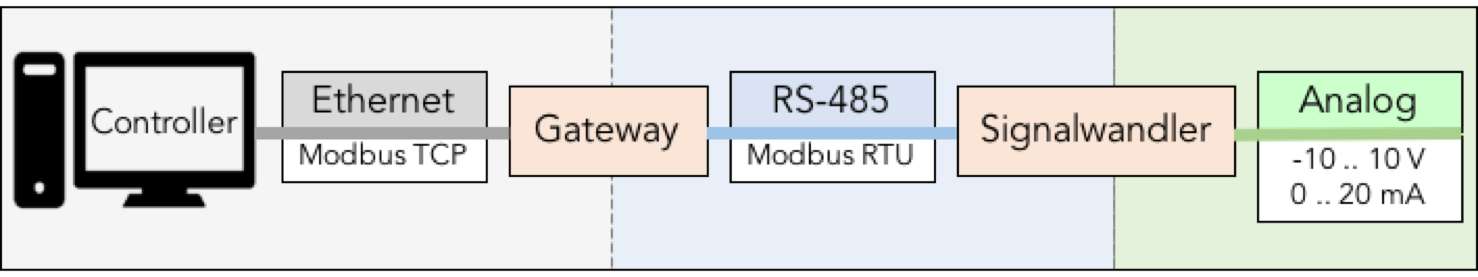
\includegraphics[width=\textwidth]{abbildungen/20160324_netzwerk}
\caption{Aufbau des Netzwerks}
\label{fig:netzwerk}
\end{figure}

\subsection{Erfassung der Raumtemperatur}

Die Raumtemperatur kann einfach und preiswert mithilfe von Raumtemperaturfühlern gemessen werden. Der Messwert soll anschließend über eine der beiden Modbus Schnittstellen dem Controller zur Verfügung gestellt werden. Innerhalb der Anlage kommen zwei \textsc{THERMASGARD RTM1-Modbus} Raumtemperaturfühler ohne Display von \textsc{S+S Regeltechnik} zum Einsatz, da sich diese aufgrund weiterer vorteilhafter Eigenschaften, wie zum Beispiel ihrer Kalibrierfähigkeit, auszeichnen. Die detaillierten Funktionen und Daten der Raumtemperaturfühler können dem Datenblatt im Anhang \ref{att:rtm1} entnommen werden.

Ursprünglich sollten die beiden Temperatursensoren auf einer mittig gedachten Achse im Raum in nord-südlicher Richtung  jeweils am Ende des in der Mitte stehenden Schreibtischs platziert werden. Da jedoch während der Installation der Anlage von Seiten der Hochschule Karlsruhe vier weitere Temperatursensoren zusammen mit einem Messumformer zur Verfügung gestellt wurden, wurde eine veränderte Anordnung der Sensoren gewählt. 
Bei den Sensoren handelt es sich um vier PT1000 Temperatursensoren, die über den \textsc{Webthermograph 8x} von \textsc{WuT} die Messwerte zur Verfügung stellen. Da der Webthermograph keine Modbus Schnittstelle besitzt, wird er über ein Netzwerkkabel in das Ethernet Netzwerk integriert und kann unter Verwendung des HTTP Protokolls vom Controller ausgelesen werden.
Um Messwerte mit dem Controller auszulesen, bietet sich das Python Paket \textit{httplib} an, welches das HTTP Protokoll implementiert und Grundfunktionen zur Verfügung stellt. 
Als veränderte Anordnung der Temperatursensoren wurden jeweils drei Sensoren an den gegenüberliegenden Wänden Richtung Osten und Westen platziert. Die Sensoren wurden entlang der westlichen Außenwand und der östlichen Innenwand gleichmäßig verteilt und auf einer Höhe von 2~m installiert. Die Identifizierung der Sensoren erfolgt über ID´s, die zusammen mit ihrer Anordnung in \ref{fig:raumtempsensors} visualisiert sind.

\begin{figure}
\centering
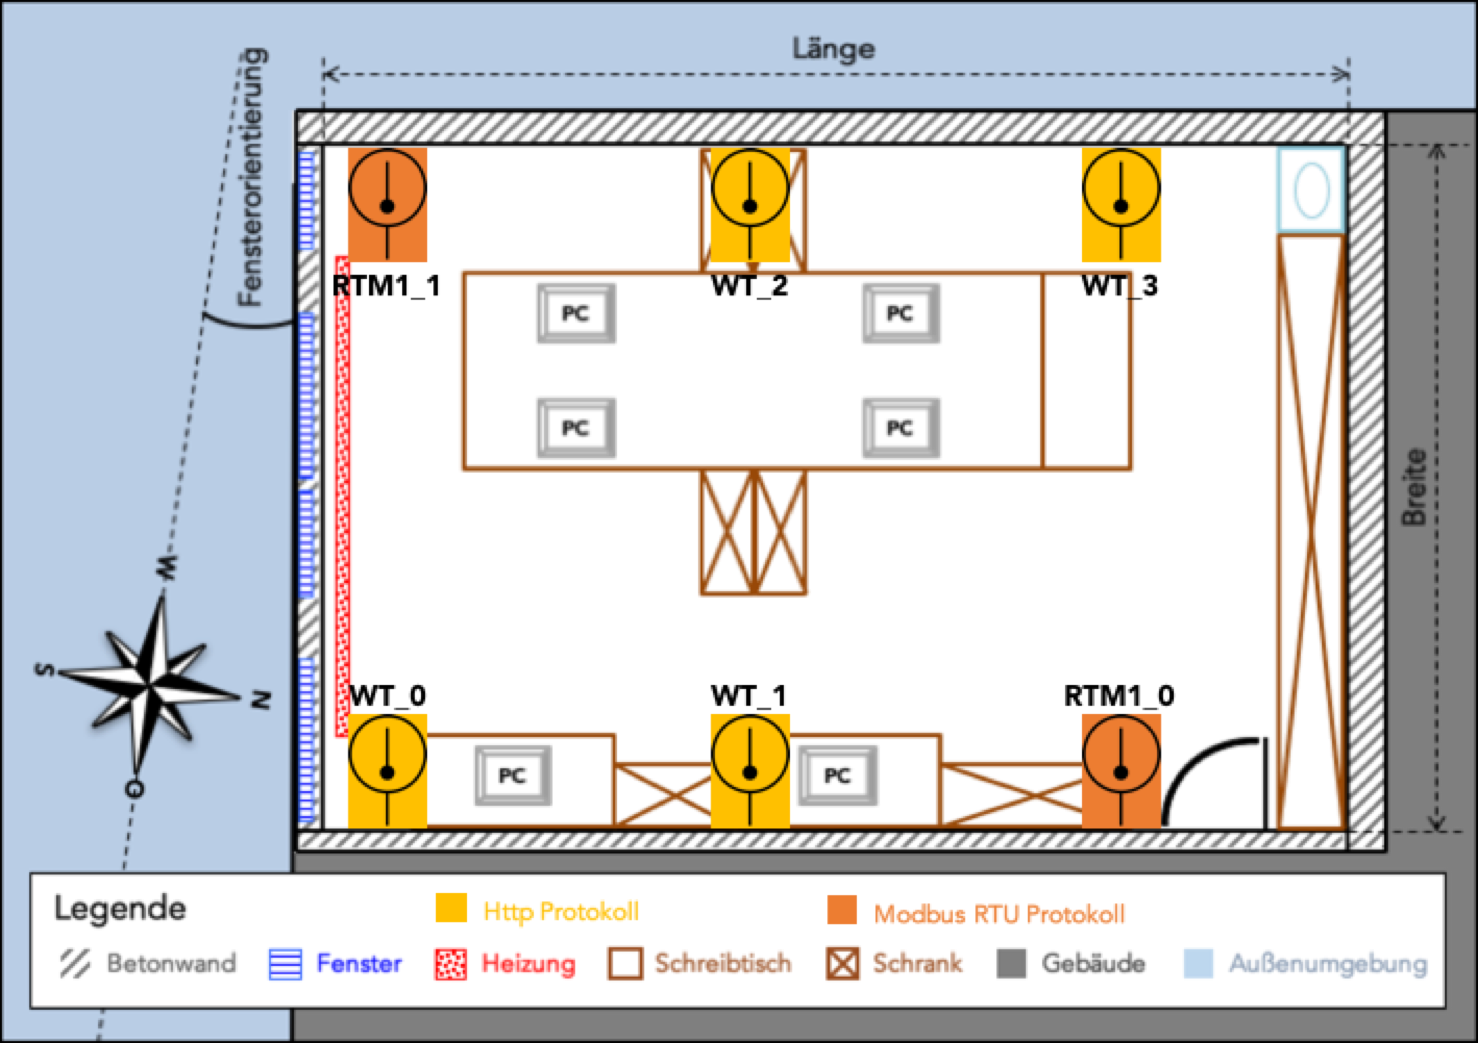
\includegraphics[width=\textwidth]{abbildungen/20160324_sensors}
\caption{Verteilung der Raumtemperaturfühler}
\label{fig:raumtempsensors}
\end{figure}

\subsection{Steuerung des Heizkörpers}

Um die Heizung mit den benötigten Sensoren auszustatten, bietet sich wie in Abschnitt \ref{sub:idee} erwähnt ein Wärmemengenzähler an. Die Temperaturmessung am Ein- und Auslass der Heizung gestaltet sich jedoch etwas aufwendiger als zuvor. Es werden Tauchhülsen im Vor- und Rücklauf des Heizkörpers benötigt, welche vom Heizwasser direkt umflossen werden. Aufgrund der Tauchhülsen werden geringfügige bauliche Änderungen nötig, beispielsweise können diese in einen Kugelhahn eingeschraubt werden. Sie sind jeweils mit einem Temperaturfühler bestückt und ermöglichen dadurch die Messung der Heizwassertemperatur. Der Einbau des Durchflusssensors erfordert ebenfalls bauliche Maßnahmen. Dazu wird entweder im Vor- oder Rücklauf, je nach Spezifikation Herstellers, ein Stück Rohrleitung entfernt und durch den Durchflusssensor ersetzt. Dieser kann beim Einbau entweder fest integriert oder durch eine Anschlussverschraubung, beziehungsweise einen Flanschanschluss, demontierbar eingebaut werden.

In der Anlage kommt der Wärmemengenzähler \textsc{MULTICAL 602} von \textsc{Kamstrup} zum Einsatz, da er neben einem geforderten Modbus Kommunikationsmodul weitere besondere Eigenschaften mit sich bringt. Die Temperaturmessung erfolgt durch zwei PT500 Sensoren, wohingegen der Durchfluss von einem \textsc{ULTRAFLOW 54} Ultraschallsensor erfasst wird. Die gemessenen, wie auch die berechneten Werte der Heizungsleistung lassen sich einzeln durch das Rechenwerk auslesen.
Der \textsc{MULTICAL 602} ist zum einen kostengünstig und umfasst alle benötigten Sensoren, die bereits präzise aufeinander abgestimmt sind. Zum anderen ist er wartungsfrei, da er den Durchfluss über kontaktlose Ultraschallmessungen bestimmt, indem er die Laufzeitdifferenz zwischen wechselseitig gesendeten und empfangenen Signalen zweier integrierter Ultraschallsensoren auswertet. Ein klarer Vorteil des Durchflusssensors \textsc{ULTRAFLOW 54} ist, dass er bereits mit einer Tauchhülse ausgestattet ist, sodass lediglich eine weitere Tauchhülse montiert werden muss.


Die Steuerung des Durchflusses im Heizkörper erfolgt über ein Heizungsventil, welches mithilfe eines Stellantriebs geöffnet und geschlossen wird. Dieser kann wiederum von einem Elektromotor angetrieben werden, der sich durch seine schnelle Reaktion, jedoch auch durch seine hohen Anschaffungskosten auszeichnet. Alternativ kann ein thermoelektrisches Element als Antrieb genutzt werden, welches sich durch seine geringen Anschaffungskosten auszeichnet, allerdings aber eine langsamere Reaktionszeit besitzt. Die Ansteuerung des Stellantriebs erfolgt üblicherweise unabhängig von der Ausführung durch ein digitales oder analoges Spannungs- oder Stromsignal.

Um eine Steuerung durch den Controller zu ermöglichen wird ein Signalwandler eingesetzt, der Modbustelegramme in elektrische Signale umwandeln kann. Hierzu wird innerhalb der Anlage das \textit{EX9024-M} Modul von \textsc{ExpertDAQ} integriert, welches sich leicht in ein serielles RS485-Netzwerk einbinden lässt. Das Modul ist Modbus RTU-fähig und besitzt vier analoge Ausgänge, die verschiedene Spannungs- und Strombereiche ausgeben können. Da für den Stellantrieb lediglich ein Ausgang genutzt wird, besteht die Möglichkeit einer einfachen Erweiterung der Anlage um drei weitere analoge Komponenten, wie beispielsweise einen Schalter zur Bedienung der Jalousien.

Der thermoelektrische Stellantrieb \textit{ABNM-LIN} von \textit{Danfoss} wird zur stufenlosen Betätigung des Heizkörperventils eingesetzt. Seine Ansteuerung erfolgt über ein analoges 0-10~V Signal, welches innerhalb der Anlage vom EX9024-M bereitgestellt wird. Der Stellantrieb wandelt das angelegte Signal in einen proportionalen linearen Stellweg um, womit er den Durchfluss im Heizkörper steuert.


Das beschriebene Konzept zeichnet sich besonders dadurch aus, dass es eine kostengünstige Umsetzung erlaubt und obendrein eine größtmögliche Kompatibilität der Anlageteile und Bauteile sicherstellt. Die Forderung nach der Erweiterbarkeit der Anlage wird explizit durch die offene Architektur und die Wahl der eingesetzten Komponenten berücksichtigt, sodass langfristig die Möglichkeit besteht ganzjährig die Raumtemperatur regeln zu können, beispielsweise unter Zuhilfenahme einer Raumklimatisierung und der Ansteuerung der Jalousien.

\section{Installation und Inbetriebnahme}

Eine Übersicht über den Aufbau der Anlage findet sich in Abbildung REFXXXXX. Die Installation lässt sich in die zwei Bereiche Hardware und Software untergliedern. Die Hardware Installation umfasst die  Montage der einzelnen Komponenten, deren Stromversorgung und die Verkabelung im Netzwerk.
Der zweite Teil beschäftigt sich mit der Inbetriebnahme der Anlage durch eine softwareseitige Ansteuerung der Anlage.


\subsection{Hardware}

Der Aufbau des Netzwerks wurde bereits in \ref{fig:netzwerk} dargestellt. Als Ethernet-Netzwerk wird das lokale Netzwerk der Hochschule Karlsruhe genutzt. Dadurch ist eine flexible Ansteuerung der Anlage innerhalb des gesamten lokalen Netzwerks und über eine VPN-Verbindung auch außerhalb vom Campus möglich. Der Rechner ist bereits im Netzwerk integriert, sodass lediglich das Gateway beim Rechenzentrum der Hochschule Karlsruhe registriert werden musste, damit ihm eine IP~Adresse gemäß dem Ethernet/IP Protokoll zugewiesen werden konnte.
Um den Webthermographen in die Anlage einzubinden, wurde dasselbe Prozedere durchlaufen.

Der Schaltplan des seriellen RS-485 Netzwerks wird in \ref{fig:schaltplan} dargestellt. Zur Verkabelung des Netzwerks wird eine Busleitung von \textsc{LappKabel} verwendet, welche aus zwei jeweils paarweise verdrillten Leitungspaaren
besteht, die durch ein Kupfergeflecht gegen Störungen abgeschirmt sind. Das Datenblatt der Busleitung ist im Anhang unter XXXX zu finden.
Die Verkabelung erfolgt gemäß der Spezifikationen im Modbus seriell Protokoll ZITAT, daher wird die D0 Leitung der braunen Ader, die D1 Leitung hingegen der gelben Ader und die GNC Common Leitung der weißgrauen Ader zugewiesen. Das grüne Kabel kann für eine gemeinsame Stromversorgung der Komponenten eingesetzt werden, was im Rahmen dieser Anlage aufgrund der vielen unterschiedlichen benötigten Spannungen nicht genutzt wurde. Folglich hat jede Komponente, wie im Schaltplan dargestellt, ein eigenes Netzteil und daher eine eigene Stromversorgung. 

Die Kabel wurden gemäß der Übersicht in REFFFFXXXX verlegt und mit den Bauteilen entsprechend dem Schaltplan in ref{fig:schaltplan} verbunden. Die kurzen Stichleitungen wurden über flexibel einsetzbare und zugleich wiederverwendbare Hebelklemmen an die lange Busleitung angeschlossen.


\begin{figure}
\centering
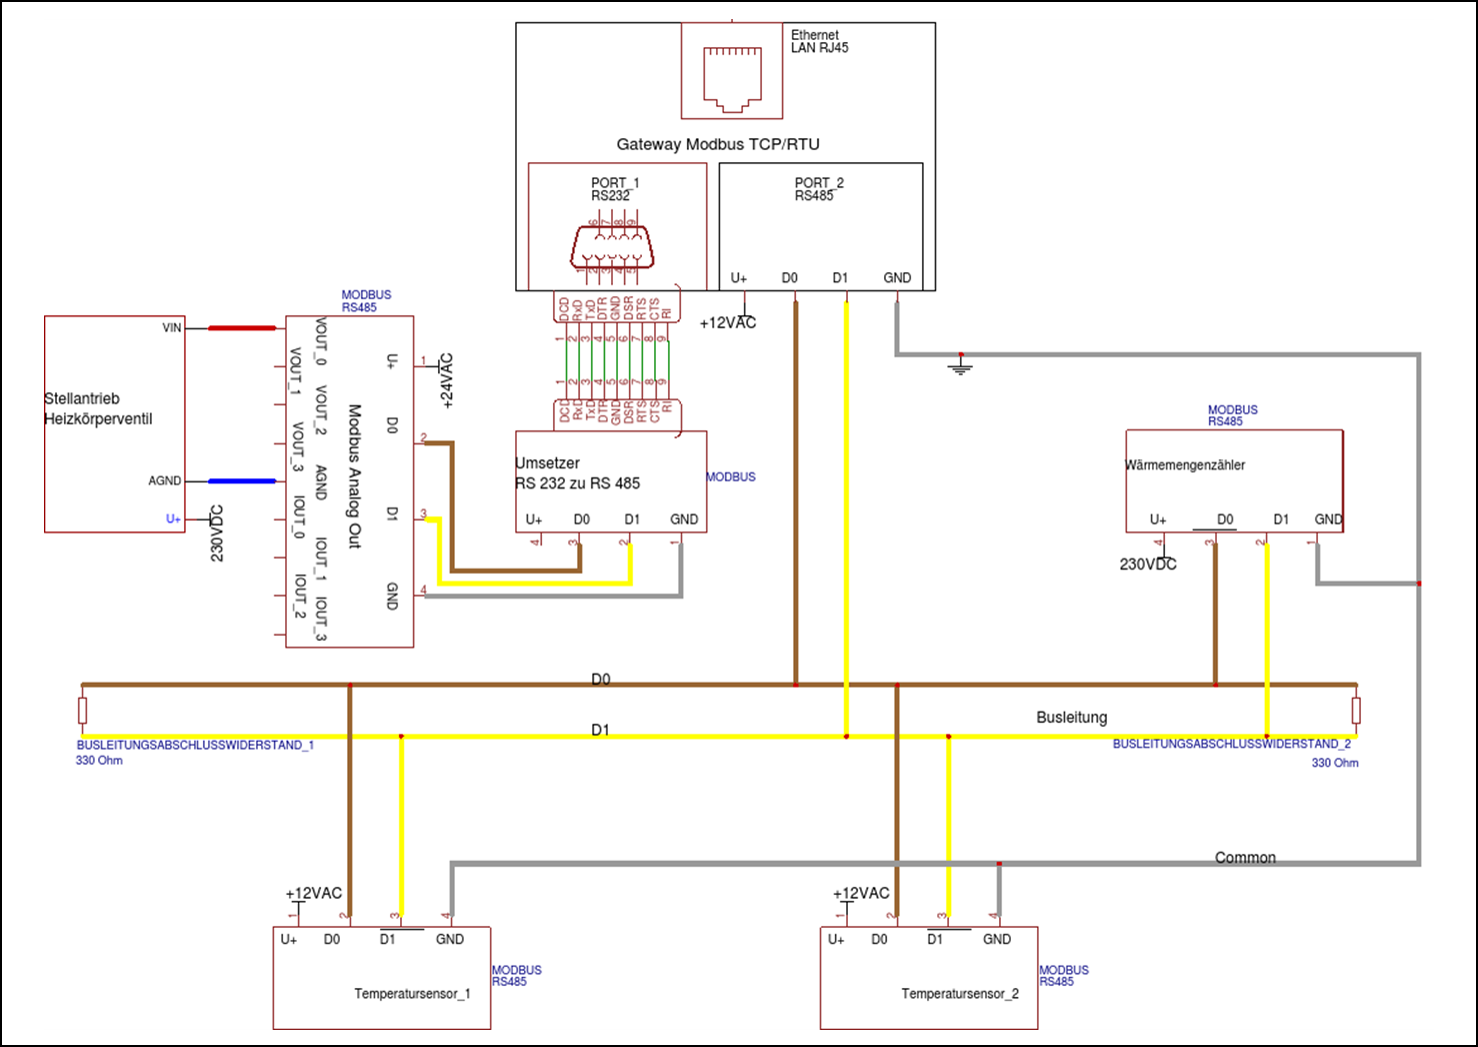
\includegraphics[width=\textwidth]{abbildungen/20160326_schaltplan}
\caption{Schaltplan der Raumtemperaturregelungsanlage}
\label{fig:schaltplan}
\end{figure}

Die Konfiguration des RS 485 Netzwerks geschieht über das Gateway, dessen Einstellungen in Tabelle \ref{tab:konfport} abgebildet sind.

\begin{table}[H]
\centering
\small
\renewcommand{\arraystretch}{1.3}
\begin{tabularx}{1\textwidth}{m{0.3\textwidth}m{0.3\textwidth}m{0.3\textwidth}}

\toprule

\textbf{Konfigurationsmerkmal} & \textbf{Werte Port 1} & \textbf{Werte Port 2} \\

\cmidrule[0.5pt](r{0.25em}){1-1} 
\cmidrule[0.5pt](l{0.25em}){2-2}
\cmidrule[0.5pt](l{0.25em}){3-3}

Port & 502\\

\ccol Baudrate & \ccol	19200 [$\frac{bits}{S}$]& \ccol	9600 [$\frac{bits}{S}$]	\\

Parität	& Gerade & Keine		\\

\ccol Datenbitlänge & \ccol 8 & \ccol 8	\\

Stoppbits & 1 &	1	\\

\ccol Timeoutzeit &	\ccol 10 [$mS$] & \ccol 10 [$mS$]	\\

Betriebsweise 	&	Modbus TCP zu RTU\newline Server &	Modbus TCP zu RTU\newline Server \\


\bottomrule
\end{tabularx}
\caption{Netzwerkkonfiguration der Ports des EX9132M-MTCP Gateways}
\label{tab:konfport}
\end{table}


Bei der Inbetriebnahme der Anlage kam es zu Schwierigkeiten bei der Kommunikation. Es stellte sich heraus, dass der Signalwandler EX9024M nicht streng nach den Modbus Spezifikationen für serielle Kommunikation hergestellt wird. Infolgedessen kann dieser nicht mit den beiden Raumtemperaturfühlern innerhalb eines Netzwerks betrieben werden,da keine kompatible Netzwerkkonfiguration zustande kommt. Das Gateway ist mit zwei Ports ausgestattet, wovon der zweite zum Aufbau eines weiteren seriellen Netzwerks genutzt wird und dadurch das Problem beseitigt wurde. Hierfür wurde ein Bridge, in der Form eines einfachen Adapters, genutzt, der die Spannungspegel und Steckerbelegungen des RS 232 Ports auf die einer RS 485 Schnittstelle umsetzt. Hierzu findet sich eine Darstellung im Schaltplan in \ref{fig:schaltplan}.


\subsection{Software}

Um eine zentral Steuerung vom Controller aus zu gewährleisten, müssen verschiedene Schnittstellen zu Python von einzelnen Komponenten der Anlage genutzt werden.
Wie bereits erwähnt, bietet Python verschiedene Pakete an, die Funktionalitäten bereitstellen. Nichtsdestotrotz muss eine eigene anlagenspezifische Software entwickelt werden, die zu einem gewissen Teil auf die von Python bereitgestellten Funktionalitäten zugreift. Der im Folgenden beschriebene Programmcode erfolgt vollständig objektorientiert und versucht eine klare Struktur und Wiederverwendbarkeit einzelner Methoden und Klassen zu gewährleisten. Das oberste Ziel der Programmierung war es, eine einfache Bedienbarkeit der Anlage, sprich eine Bedienung ohne Kenntnisse über die zugrundeliegende Kommunikationstechnik, zu ermöglichen.

Zum Auslesen der vier Temperatursensoren über den Webthermograph8x wurde das Python Paket httlib genutzt. Die Abfrage der Temperatursensoren über das HTTP Protokoll wurde in einer eigenen Klasse SensorsHttp implementiert, welche das HTTPConnection Objekt aus der httplib verwendet. Die konkrete Umsetzung der Klasse ist in Listing \ref{lst:webtemp} dargestellt.

Um eine Verbindung zum Thermograph8x herzustellen wird dessen IP Adresse und Port Nummer benötigt, über die Telegramme gesendet und empfangen werden. Die Werte hierfür sind aus Gründen des Zugriffsschutzes nicht im Programmcode hinterlegt, sondern finden sich in den Umgebungsvariablen server-address und server-port der Pythonkonsole des Controllers wieder.
Mithilfe der init-Methode wird bei der Initialisierung ein HTTPConnection Objekt server erstellt, dem als Host und Port die Adressen des Webthermographen übergeben werden.
Des Weiteren wird jeweils eine Methode zur Herstellung und zur Trennung der Verbindung definiert, sowie eine abstrakte Methode get-wt, welche die allgemeine Abfragesyntax der Messwerte enthält. Die Messwerte können lediglich einzeln durch eine Serveranfrage abgefragt werden, welche die Messwerte durch einen einfachen Befehls-string \Gun GET\textbackslash Single \Gob zusammen mit der ID des gewünschten Temperatursensors anfordert. Nach erfolgter Rückgabe des Messwerts, der in einen float Datentyp umgewandelt wurde, wird die Verbindung zum Server wieder getrennt. Die Methoden, die das Auslesen der einzelnen Messwerte veranlassen, rufen lediglich die abstrakte Methode auf und übergeben dabei die ID des gewünschten Temperatursensors.

\lstinputlisting[language=Python ,caption={Klasse SensorsHttp zur Abfrage der Temperaturen vom Webthermograph8x}, label=lst:webtemp]{listings/sensors_http.py}

Für die Kommunikation mit den Modbus Komponenten stehen drei verschiedene Python Pakete zur Verfügung. Eines davon heißt Minimalmodbus, da es jedoch keine Unterstützung für das Mobus TCP Protkoll bietet soll diesem keine weitere Beachtung zukommen. Nach einer ausführlichen Recherche über die beiden verbleibenden Pakete, fiel die Entscheidung auf das sogenannte pymodbus Paket. Es konnte durch seinen größeren Funktionsumfang und seine ausführlichere Dokumentation, die mit einfachen Beispielen veranschaulicht ist, überzeugen.
Um eine Kommunikation über Modbus zu ermöglichen,  wurde mithilfe des pymodbus Pakets die Klasse ModbusConnection  programmiert, die in \ref{lst:modconnect} zu sehen ist.

Für eine Kommunikation über das Modbus TCP Protokoll, bedarf es zunächst einer Verbindung zwischen Client und Server. Hierzu wird das ModbusClient Objekt genutzt, da der Controller als Client über das Modbus TCP Protokoll Anfragen an die Server stellt. Faktisch stellt der Controller ausschließlich Anfragen an das Gateway, welches die Telegramme in das serielle Modbus RTU Protokoll übersetzt, um mit den Slaves im seriellen Netzwerken zu kommunizieren. Bei der Initialisierung werden erneut die IP Adresse client-adress und der Port client-port benötigt, über die die Kommunikation stattfindet. Auch hier wurden eigene Methoden zum Aufbauen und Trennen einer Verbindung implementiert, welche bei der Initialisierung genutzt werden. Eine Besonderheit stellt die delete-Methode dar, die im Falle eines Fehlers oder beim Sterben einer Instanz der Klasse die Verbindung trennt. 
Außer den oben genannten Methoden, sind weitere für die benötigten Zugriffe auf die verwendeten Datentabellen implementiert. Die Methoden ermöglichen das Auslesen von input- und holding-registers und liefern ein register zurück, welches in Abhängigkeit des jeweiligen betrachteten Datenmodells einen bestimmten Datentyp besitzt. Für die beiden Lesemethoden wird eine Anfrage maximal zehn Mal wiederholt, wobei nach jedem Fehlversuch eine Pause von 1,5 Sekunden vorgesehen ist. Für die Abfrage wird die Datenadresse der jeweiligen Tabelle, die Anzahl der auszulesenden Register sowie die Slave-ID benötigt. Die letzte Methode zum Schreiben in Register wird auf drei Fehlversuche begrenzt, die ebenfalls durch eine Pause von 1,5 Sekunden voneinander getrennt sind. Auch hier wird die Datenadresse und die Slave-ID benötigt, um den mitgegebenen Wert in die Tabelle zu schreiben.
Damit sind die grundlegenden Funktionen für eine Modbus Kommunikation implementiert.

\lstinputlisting[language=Python ,caption={Klasse zum Verbindungsaufbau und für die Grundfunktionen über Modbus TCP}, label=lst:modconnect]{listings/modbus_connection.py}

Die Grundfunktionen werden von der SensorsModbus Klasse genutzt, um diverse Messwerte von den verschiedenen Sensoren abzufragen. Der zugehörige Code ist in Listing \ref{lst:modread} abgebildet.
Beim Auslesen der Werte aus dem Wärmemengenzähler findet sich eine Besonderheit, da dessen Messwerte die Größe eines einzelnen Registers übersteigen. Wie in Abschnitt XXXXX erwähnt, werden die Daten gemäß der Big-Endian Codierung verschlüsselt und müssen daher decodiert werden. Dazu bietet pymodbus mit dem BinaryPayload Decodierereine eine passende Funktion an. Hierbei muss berücksichtigt werden, dass die Decodierung von Little- und Big-Endian in pymodbus vertauscht sind. Zum Auslesen der Messwerte im Wärmemengenzähler werden der Count, der die Anzahl der zu lesenden Register angibt, und die ID des Bauteils im seriellen Netzwerk angegeben. Die konkreten Messwerte unterscheiden sich durch ihre Adressen in den Datentabellen und sind in den entsprechenden Methoden hinterlegt. 
Eine Übersicht der Adressen findet sich in den Datenblättern der Bauteile im Anhang refXXXXXXXXX.
Die beiden Temperatursensoren geben die Temperatur in Form eines ganzzahligen Werts zurück, der um eine Zehnerpotenz erhöht ist. Daher müssen die abgefragten Werte durch eine Division durch zehn decodiert werden. Die Messwerte der zum Zeitpunkt der Abfrage herrschende Raumtemperatur, stehen unter der gleichen Tabellenadresse, müssen jedoch anhand ihrer jeweiligen Sensor ID aus den zugehörigen Tabellen ausgelesen werden. Die IDs wurden den Temperatursensoren durch die Schalterstellung gemäß dem Datenblatt in refXXXXXXX zugewiesen.

\lstinputlisting[language=Python ,caption={Klasse zum Auslesen über Modbus TCP}, label=lst:modread]{listings/sensors_modbus.py}

Die Klasse AcuatorsModbus erweitert ebenfalls die ModbusConnection Klasse, allerdings um die Aktuatoren anzusteuern. Dazu wird der Spannungsausgang am EX9024M mithilfe der dezimalen Registerwerten zwischen 8191 und 16383 gesteuert, die sich aus den Hexadezimalwerten im Datenblatt REFXXX ergeben. Der Maximalwert entspricht einer Ausgangsspannung von 10 V, der Minimalwert entsprechend 0 V. Im Rahmen der Anlagensteuerung soll jedoch nicht die Ausgangsspannung, sondern die Ventilstellung gesetzt werden. Um die Ventilstellung opening-level direkt anzugeben, 0 für Ventil zu und 1 für voll offen, erfolgt eine Umrechnung, zunächst in den entsprechenden Spannungswert und anschließend in den Registerwert der in die Datentabelle geschrieben wird. Außerdem wurde eine Methode zur Abfrage der Ventilstellung implementiert.

\lstinputlisting[language=Python ,caption={Klasse zum Auslesen über Modbus TCP}, label=lst:modact]{listings/actuators_modbus.py}

Es wurden zwei weitere Klassen implementiert, die die vorausgegangenen Sensor und Aktor Klassen ein letztes Mal erweitern. Sie dienen dazu eine Bedienoberfläche zu schaffen, die sowohl unabhängig von ihrer Plattform als auch von ihrer Kommunikationstechnologie ist. Die Klassen Sensors und Actuators bewerkstelligen dies, indem sie die zuvor definierten Klassen importieren und bei der Initialisierung jeweils eine Instanz der Klasse bilden. Um eine Unabhängigkeit von der Kommunikationstechnologie zu erreichen, wird für jeden einzelnen Messwert eine eigene Methode mit eindeutiger Bezeichnung der Funktion und des Geräts definiert, ohne dass ersichtlich ist welche Kommunikation dahinter steckt. Damit ist ein Interface geschaffen, das für Steuerungen genutzt werden kann.

\lstinputlisting[language=Python ,caption={Die Actutators und Sensors Klassen zur Bedienung der Anlage}, label=lst:anlage]{listings/actuators.py}

\subsection{Inbetriebnahme mit einem Zweipunktregler}

Ein erstes, vergleichsweise einfach gehaltenes Programm zur Regelung soll die Funktion der Anlage überprüfen und dabei erste Messdaten sammeln. Anhand des Programmablaufs soll im Folgenden die Ansteuerung der Anlage und das Zusammenspiel der Komponenten veranschaulicht werden.

Eine Darstellung des Programms findet sich in Listing \ref{lst:oven}. Es zeigt die Implementierung eines simplen Zweipunktreglers, der nach dem bekannten Backofenprinzip arbeitet. Der Zweipunktregler besitzt eine Schalthysterese von einem Grad Celsius. Zunächst werden die beiden Bedienoberflächen Sensors und Actuators, gemeinsam mit einem Paket zum einfügen von Messwerten in eine Datenbank, importiert. Anschließend werden die verschiedenen Verbindungsparameter aus den Umgebungsvariablen der Pythonkonsole ausgelesen und zum Aufbau einer Verbindung mit den Anlagenteilen und der Datenbank genutzt. Dies geschieht durch die Instanziierung der Bedienoberflächenklassen Sensors und Actuators, die den Variablen s beziehungsweise a zugewiesen werden. Es folgt die Deklaration der beiden Ventilstellungen für die Schaltpunkte. 

Der eigentliche Steueralgorithmus beginnt mit einer while-Schleife. Eine dauerhafte Laufzeit des Algorithmus wird über die Schleifenbedingung $true$ erreicht, welche nur durch eine Tastenkombination oder durch das Auftreten eines Fehlers gestoppt werden kann.
 Tritt eines der beiden Abbruchkriterien ein, werden die Verbindungen zu den Anlagenteilen getrennt. Dieses Vorgehen soll eine schnelle Wiederaufnahme des Betriebs gewährleisten, da die Komponenten auf diese Weise nicht durch eine bestehende Verbindung blockiert werden.
Der Algorithmus beginnt damit alle Messwerte innerhalb der Anlage ausgelesen und daraus das arithmetische Mittel der Raumtemperaturen bestimmen. Die angenommene Raumtemperatur lässt sich ebenfalls über den Gewichtungsvektor weightings als gewichtetes arithmetisches Mittel berechnen.
Zum Auslesen der Werte, werden die Methoden des Sensors Objekts s und des Actuators Objekts a aufgerufen.
Das Abfangend von Fehlern wurde bereits in den unteren Klassen implementiert, sodass die Methoden zur Bedienung der Anlage einfach und robust aufgebaut sind. Außerdem wurden an gegebenen Stellen darauf geachtet, mögliche Fehlbedienungen  von vornherein auszuschließen. Ein Beispiel hierfür ist, dass nur real mögliche Ventilstellungen gesetzt und keine unmöglichen Werte angefordert werden können.
Anhand des berechneten Mittelwerts wird entschieden, ob der Heizkörper zur Raumerwärmung eingeschaltet, weiterhin genutzt oder abgeschaltet werden soll. Liegt die Raumtemperatur unterhalb von 21 Grad Celsius und der Heizkörper ist ausgeschaltet, so erfolgt eine Ausgabe in der Konsole. Diese besagt, dass es zu kalt ist, woraufhin das Öffnen des Heizungsventils veranlasst wird. Sobald die Temperatur über 22 Grad Celsius steigt und der Heizkörper zeitgleich eingeschaltet ist, erfolgt eine erneute Ausgabe. In dieser heißt es, dass es zu warm ist, wodurch das Heizungsventil umgehend geschlossen wird.
Bevor die Messdaten in der Konsole ausgegeben und in eine Datenbank eingefügt werden, erfolgt ein Update der Ventilstellung. Ehe der Algorithmus wieder von vorne beginnt, ist in der Steuerung eine Unterbrechung von 60 Sekunden vorgesehen.


\lstinputlisting[language=Python ,caption={Zweipunktregler Programm zur Inbetriebnahme der Anlage}, label=lst:oven]{listings/oven_greedy_db.py}

Aus Gründen der Übersichtlichkeit sind die Abhängigkeiten der Klassen untereinander in einem UML Klassendiagramm in Abbildung \ref{fig:uml} graphisch dargestellt. 
\begin{figure}
\centering
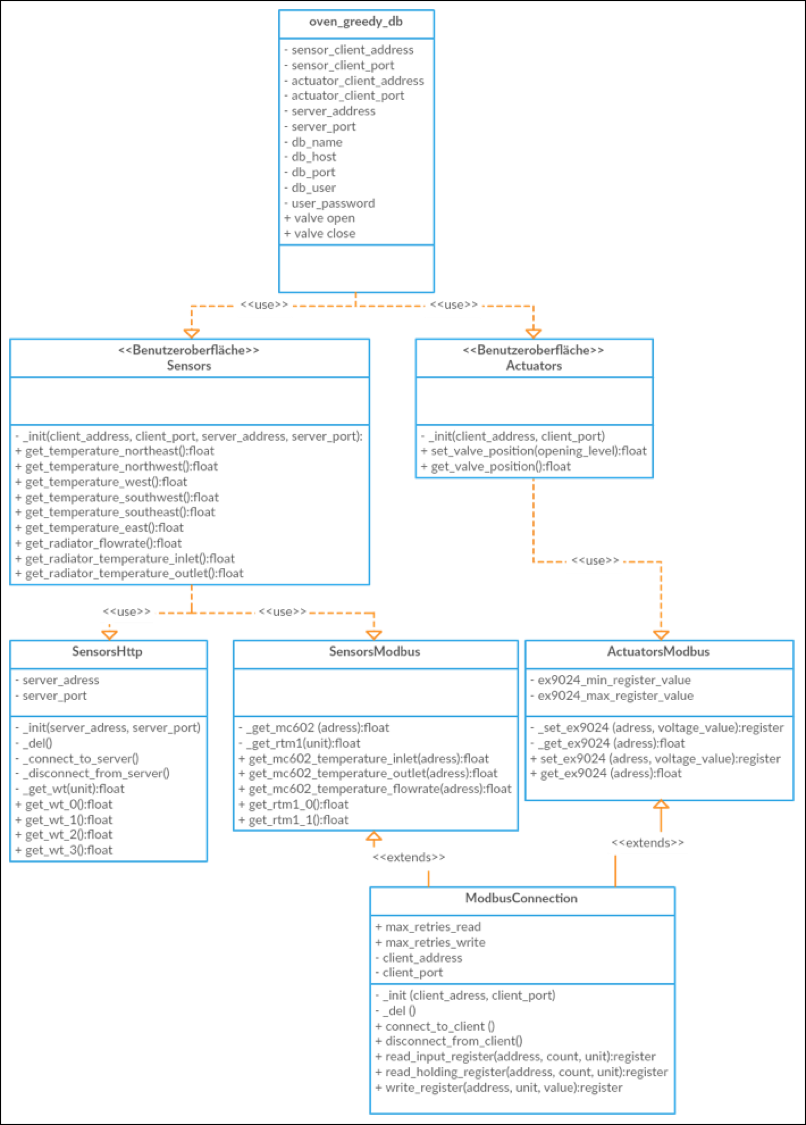
\includegraphics[width=\textwidth]{abbildungen/20160327_uml}
\caption{UML Klassendiagramm der zentralen Anlagensteuerung}
\label{fig:uml}
\end{figure}

Die Anlage konnte aufgrund von Lieferschwierigkeiten des Wärmemengenzählers erst am 16.12.2015 erfolgreich in Betrieb genommen werden. Seither sind lediglich kleinere Fehler aufgetreten, wodurch die Programmierung der Anlage stetig und sukzessive verbessert werden konnte.
Seit Mitte Januar läuft die Anlage durchgängig stabil und fehlerfrei und leistet einen sehr zuverlässigen Dienst.
Die Forderung einer hohen Funktionalität der Anlage konnte demnach erfüllt werden. Durch die Programmierung einer fehlertoleranten Software konnte ebenfalls dem Wunsch einer hohen Robustheit der Anlage nachgekommen werden.

\begin{figure}
\centering
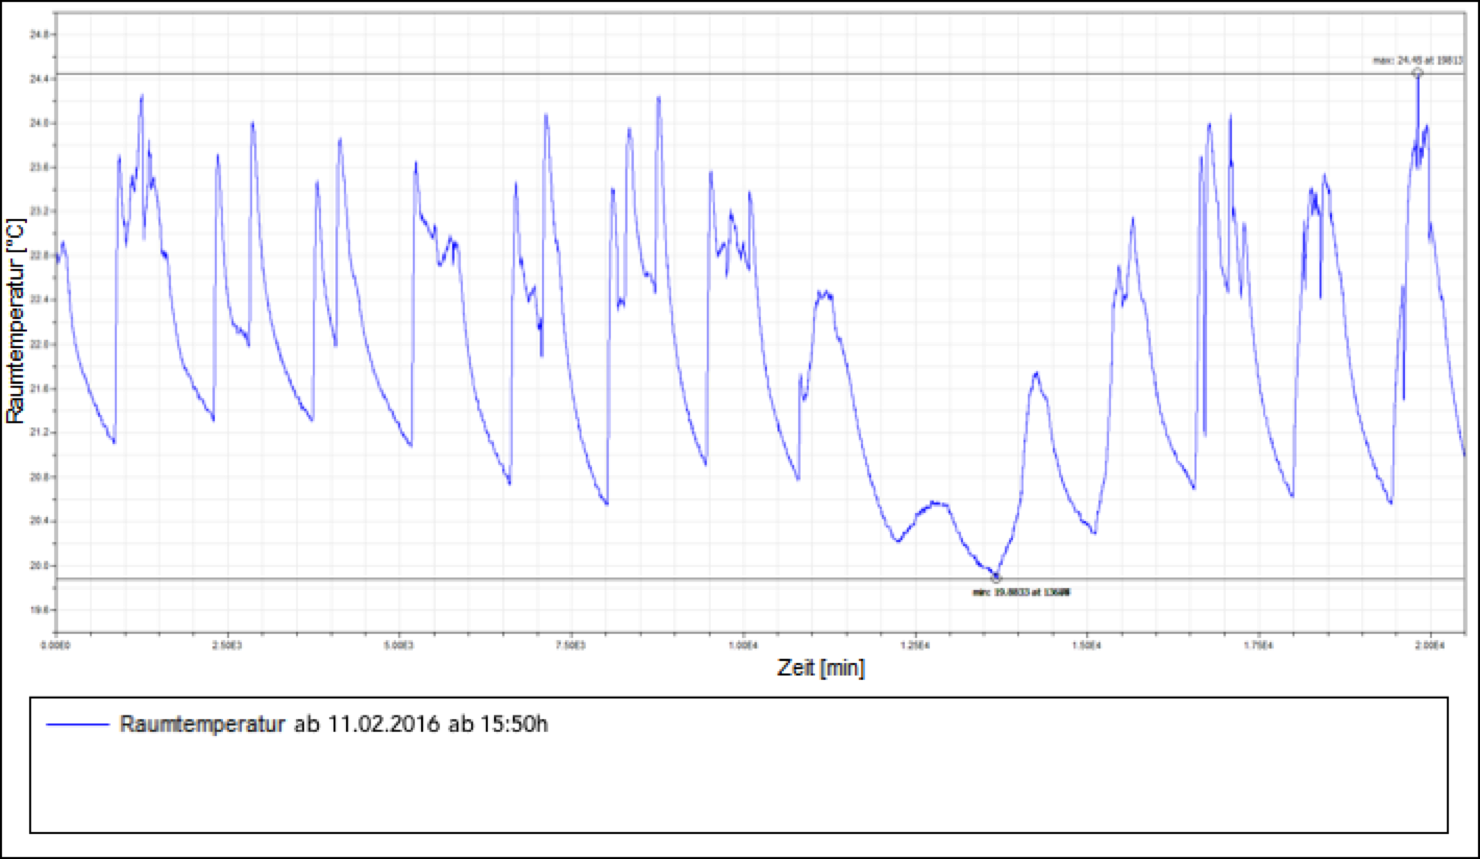
\includegraphics[width=\textwidth]{abbildungen/20160330_regelung}
\caption{Raumtemperturverlauf für ein 14-tägiges Intervall im Februar 2016}
\label{fig:regelung}
\end{figure}

Der gemessene Raumtemperaturverlauf über 14-tägiges Intervall im Februar 2016 ist in \ref{fig:regelung} dargestellt. Er wurde bei Betrieb der Anlage aufgenommen Schaltpunkte 21 und 23 Grad Durch ihn lässt sich die These bestätigen, dass die Anlage eine Raumtemperatur regeln kann.
Aufgrund der zentralen Steuerung der Anlage, welche in Python umgesetzt wurde und fehlerfrei funktioniert, sind die Voraussetzungen für eine Regelbarkeit mit Hilfe von Modellprädiktiver Regelung erfüllt. Um die Eignung zu überprüfen, wird jedoch noch ein Modell des Raumes und der Anlage benötigt, welches im nachfolgenden Kapitel gebildet wird.